\documentclass[../main.tex]{subfiles}


\begin{document}
	\section{Úvod do prostředí Robot Mesh studio}

	Našeho robota budeme programovat v prostředí Robot Mesh studio, které je zdarma dostupné na webové stránce \href{https://www.robotmesh.com/studio}{https://www.robotmesh.com/studio}. Robota lze přes toto prostředí programovat v několika jazycích, pro nás budou nejdůležitější \textbf{Blocky} a \textbf{Python}.

	V rámci této kapitoly se naučíme:
	\begin{itemize}
		\item vytvářet nové projekty,
		\item připojovat robota, aby s ním šlo v rámci prostředí komunikovat,
		\item spouštět základní programy v jazyce \textbf{Blocky}.
	\end{itemize}

	% screen shot zoom: 130%
	% firefox, with treestyle tabs

	\subsection{Vytváření nového projektu}

	Otevřete stránku \href{https://www.robotmesh.com/studio}{https://www.robotmesh.com/studio} v libovolném webovém prohlížeči.

	\begin{figure}[h!]
		\centering
		\frame{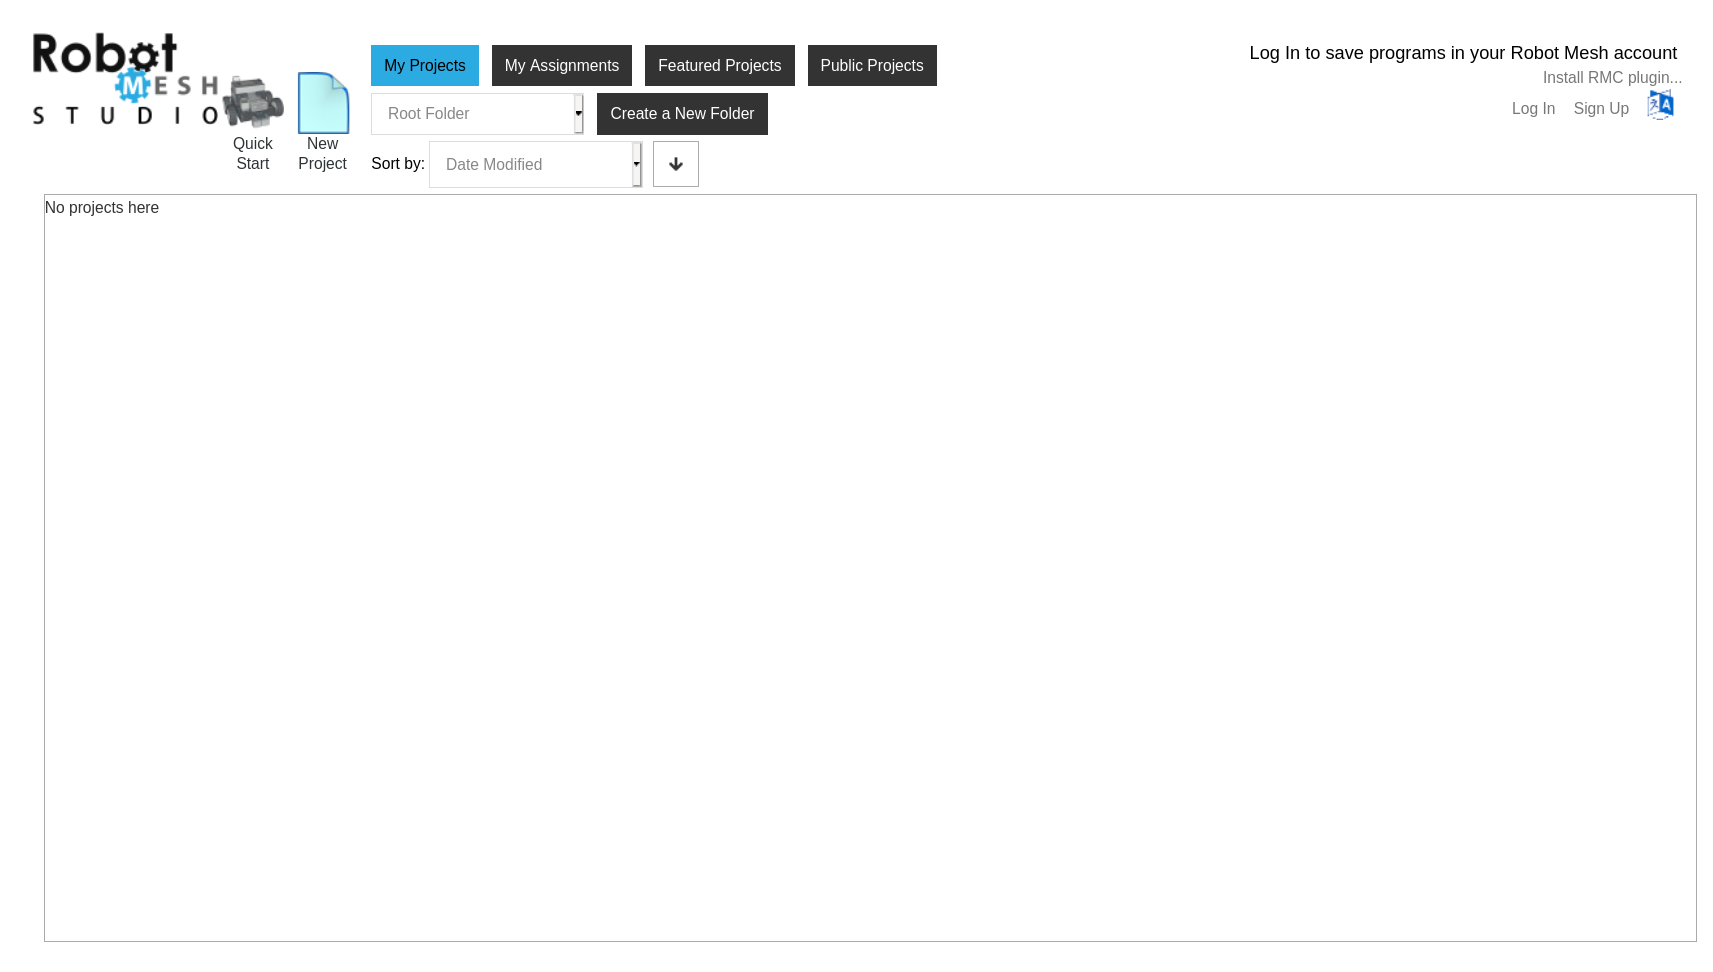
\includegraphics[width=\linewidth]{../Images/01/default-robotmesh-website.png}}
	\end{figure}

	K vytvoření nového projektu stačí kliknout na \textbf{New Project} a poté:

	\begin{figure}[ht]%
		\begin{subfigure}{.3\textwidth}%
			\centering%
			\frame{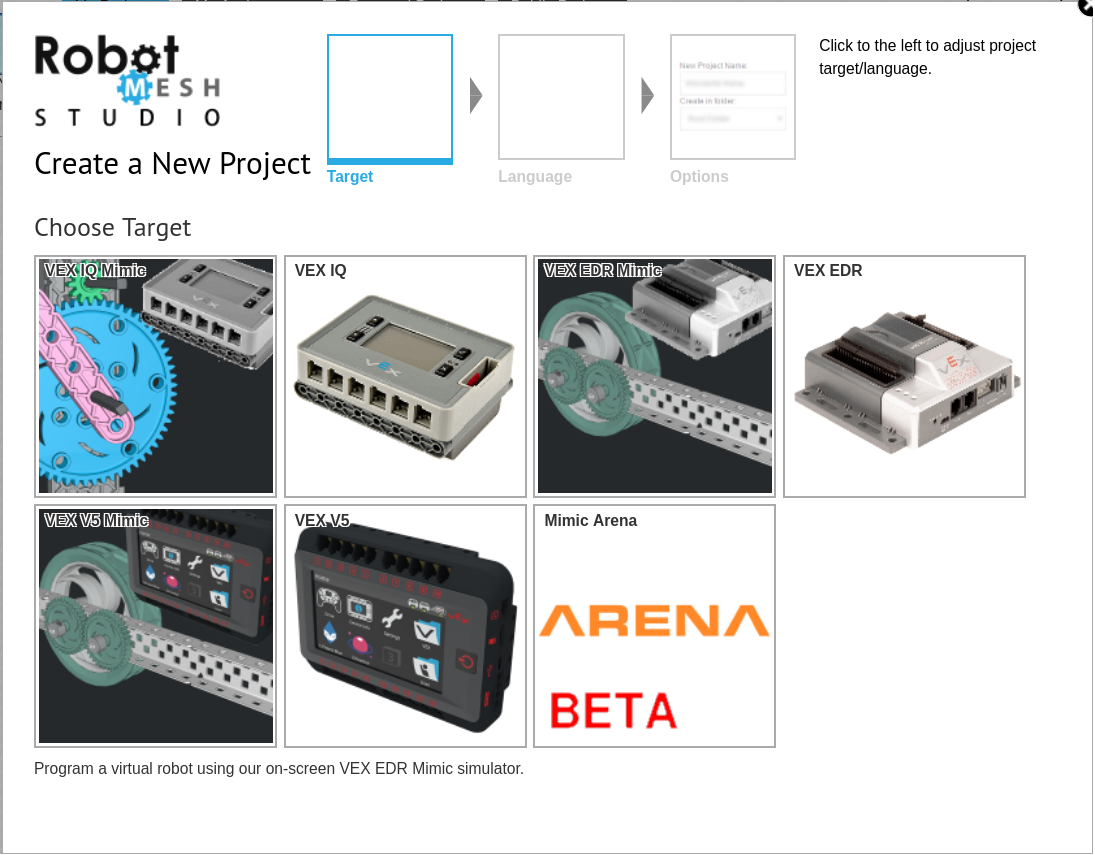
\includegraphics[width=\linewidth]{../Images/01/create-project-1.png}}%
			\caption{kliknout na \textbf{VEX V5}}%
		\end{subfigure} \hspace{.045\textwidth}%
		\begin{subfigure}{.3\textwidth}%
			\centering%
			\frame{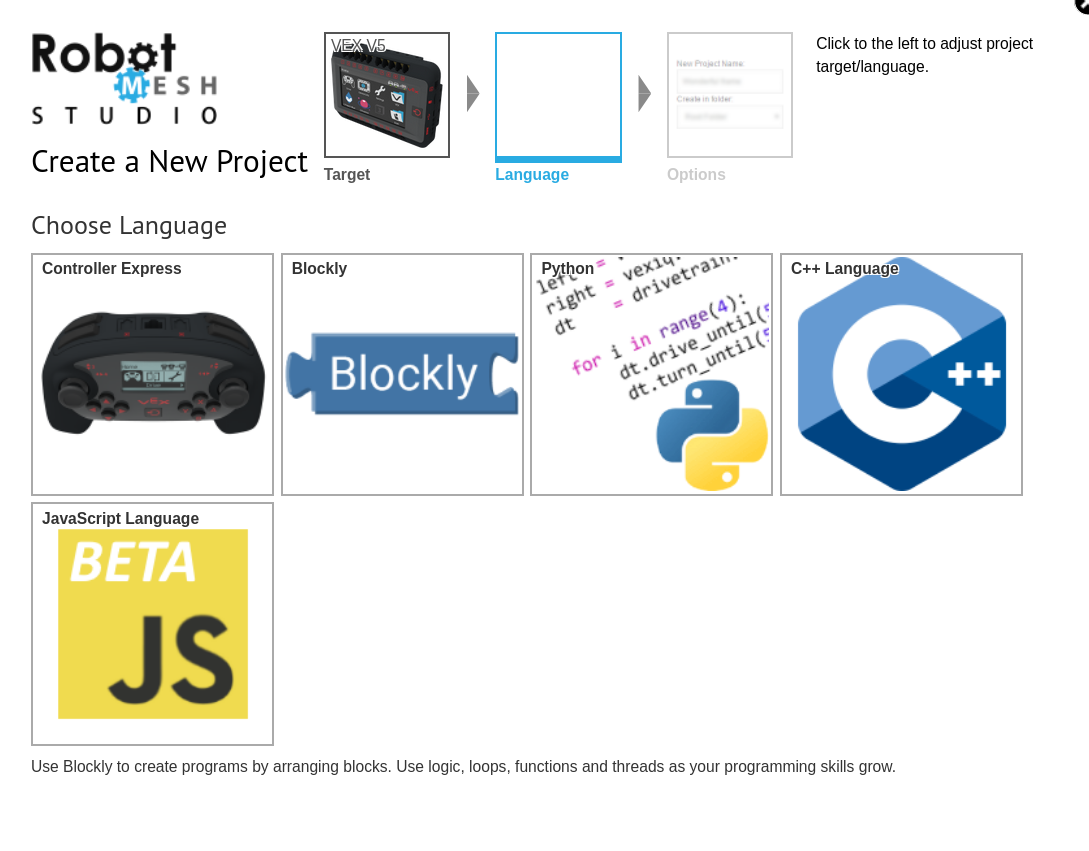
\includegraphics[width=\linewidth]{../Images/01/create-project-2.png}}
			\caption{kliknout na \textbf{Blocky}}%
		\end{subfigure} \hspace{.045\textwidth}%
		\begin{subfigure}{.3\textwidth}%
			\centering%
			\frame{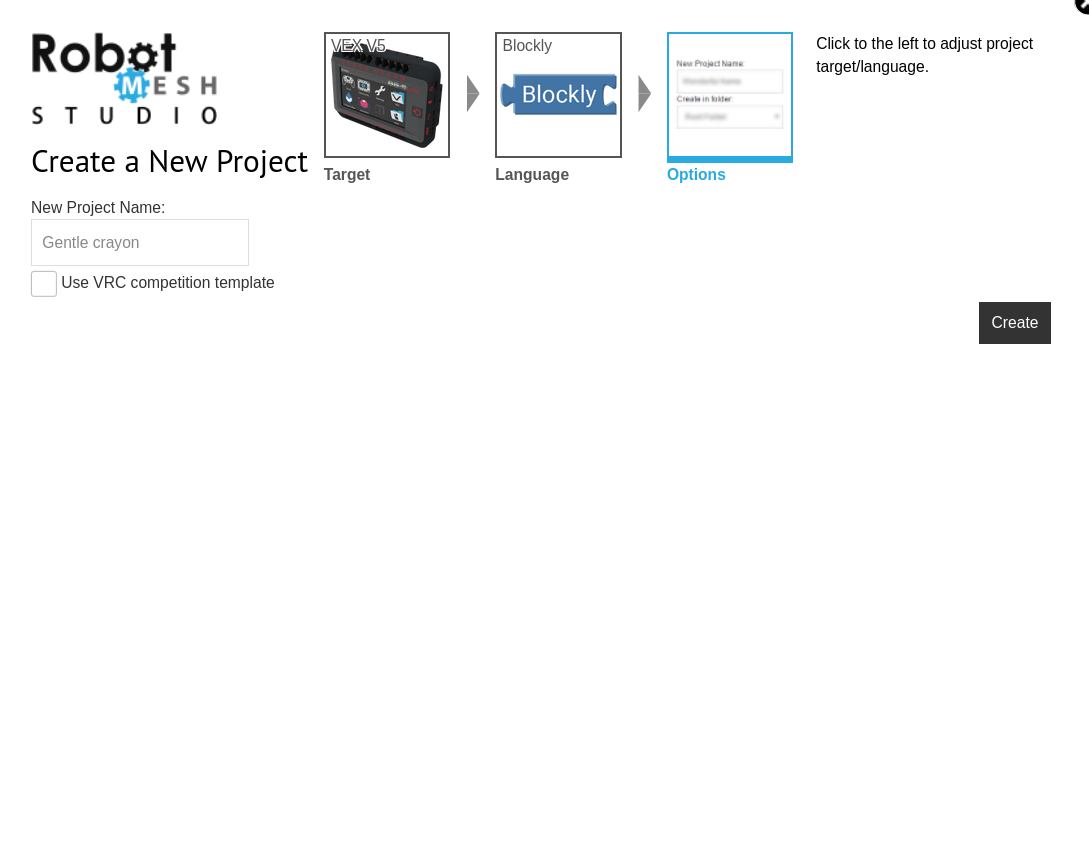
\includegraphics[width=\linewidth]{../Images/01/create-project-3.png}}%
			\caption{kliknout na \textbf{Create}}%
		\end{subfigure}%
	\end{figure}

	\newpage

	Nyní se nacházíme v samotném Robot Mesh studiu. Skládá se z několika částí:

	\begin{itemize}
		\item \textbf{Horní (ovládací) lišta} -- slouží ke spouštění, pozastavování a zastavování programu.
		\item \textbf{Levá (příkazová) strana} -- obsahuje příkazy k ovládání robota, kterými ho budeme ovládat.
		\item \textbf{Pravá (hardwarová) strana} -- TODO
		\item \textbf{Prostřední (programová) strana} -- Obsahuje samotný program.
		\item \textbf{Dolní (TODO) strana} -- TODO
	\end{itemize}

	\begin{figure}[h!]
		\centering
		\frame{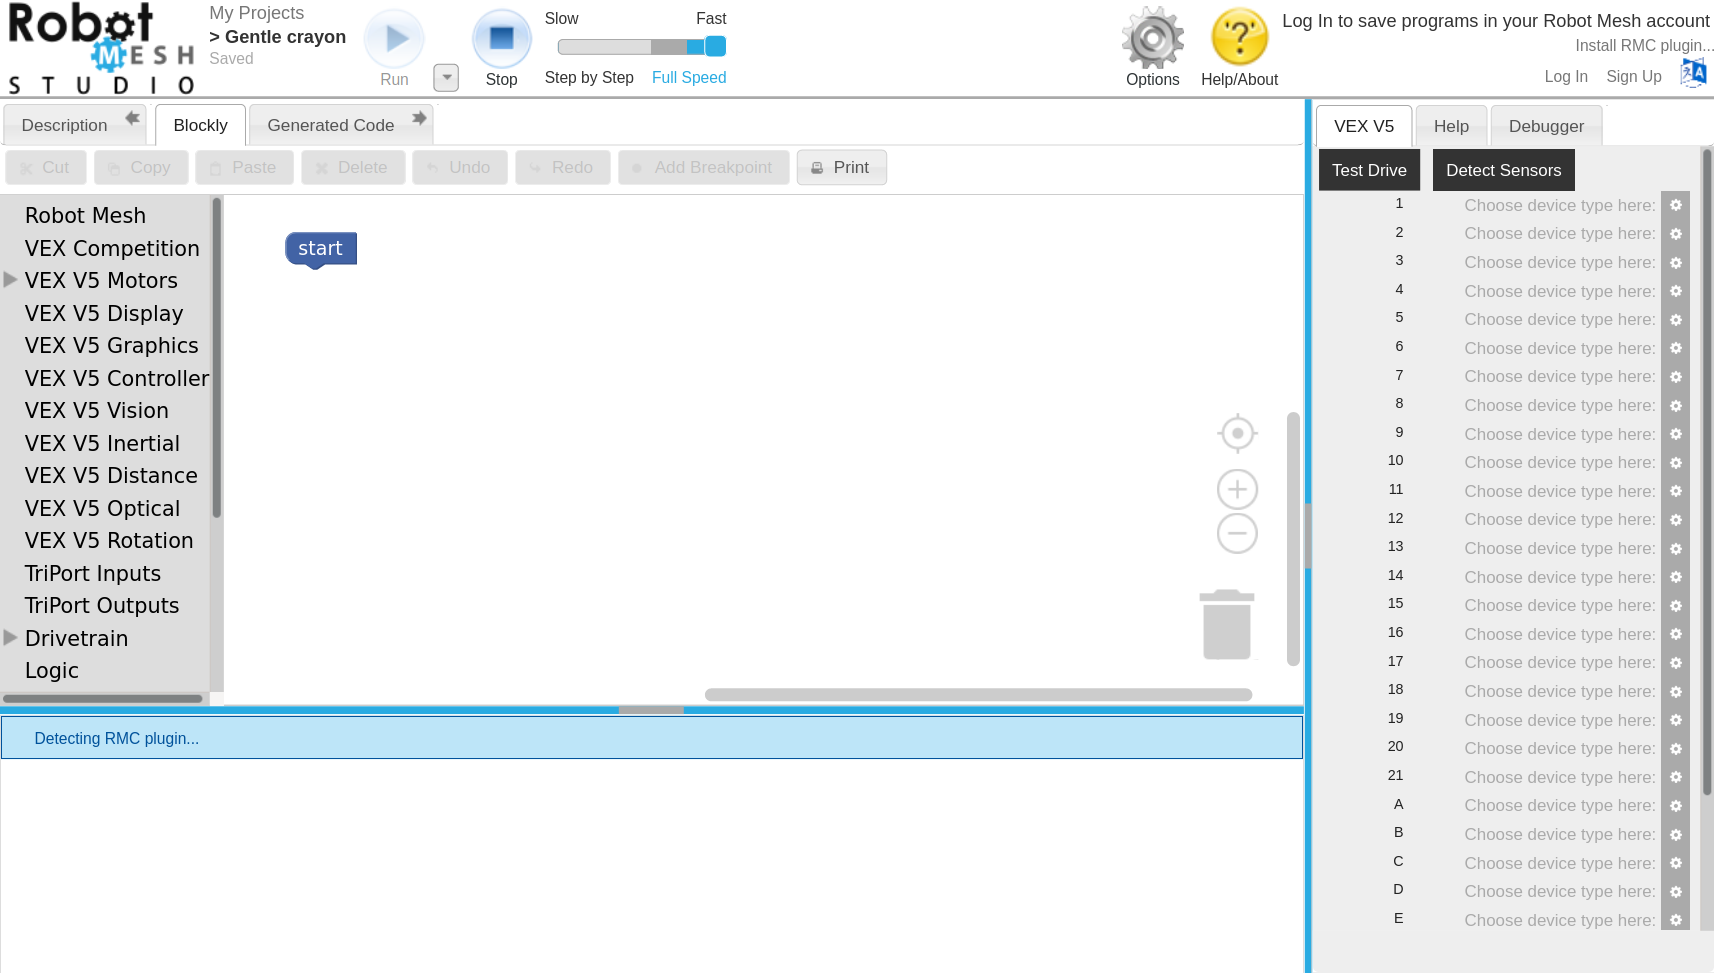
\includegraphics[width=\linewidth]{../Images/01/default-robotmesh-studio.png}}
	\end{figure}

	\subsection{Nastavení motorů a senzorů}

	TODO: připojit robota

	\subsection{Náš první Blocky program}

	Programovací jazyk Blocky funguje na principu „bloků.“ Program vždy začíná v bloku \tcbox[colback=ceruleanblue,coltext=white]{start} a vždy následuje do bloku, který je pod tím, který právě dokončil.

	

\end{document}
